\section{КЛАССИЧЕСКИЕ МЕТОДЫ ДЛЯ РЕШЕНИЯ ОДУ}

\subsection{Постановка задачи}

Программа, над которой ведётся работа, предназначена для решения дифференциальных уравнений или систем дифференциальных 
уравнений с начальными значениями, то есть задачи Коши ~--- классической математической постановки. 
Сама по себе задача достаточно сложная и изучалась уже более ста лет.

Конкретная прикладная задача сводится к решению дифференциального уравнения произвольного порядка. Общий вид такой задачи представлен
в примере \ref{eq:Koshi}.
\begin{equation}
    \begin{cases}
        y^{(n)} = f(x, y, y', y'', ..., y^{(n - 1)})\\
        y(x_0) = y_0\\
        y'(x_0) = y_1\\
        y''(x_0) = y_2\\
        ...\\
        y^{(n - 1)}(x_0) = y_{n - 1}
    \end{cases}
    \label{eq:Koshi}
\end{equation}

Данное уравнение произвольного порядка $n$ может быть преобразовано в систему из $n$ дифференциальных уравнений первого порядка путём
замены переменных. Пример \ref{eq:KoshiSystem} демонстрирует преобразование задачи Коши второго порядка в систему из 2-х уравнений
первого порядка, путём замены $y'$ на $z$:
\begin{equation}
    \begin{cases}
        z' = f(x, y, y', y'')\\
        y' = z\\
        y(x_0) = y_0\\
        z(x_0) = y_1
    \end{cases}
    \label{eq:KoshiSystem}
\end{equation}

Из курса дифференциальных уравнений известно, что задача с начальными условиями при непрерывных правых частях, удовлетворяющих условию
Липшица по всем переменным, имеет единственное решение.

Методы решения дифференциальных уравнений можно классифицировать на точные, приближенные и численные. Точные методы, которые изучаются
в курсе дифференциальных уравнений и могут быть применены к очень ограниченному кругу уравнений, позволяют выразить решение
дифференциальных уравнений либо через элементарные функции, либо с помощью квадратур от элементарных функций. К приближенным методам
относятся приемы, в которых решение дифференциального уравнения получается, как предел некоторой последовательности, элементы которой
построены с помощью элементарных функций. Численные методы представляют собой алгоритмы вычисления приближенных значений искомой
функции в узлах. %ссылку бы сюда

Такие задачи могут отличаться между собой сложностью решения. Так одни задачи можно решать при помощи группы явных методов и получать
достаточно точное решение. Другие же задачи, в которых присутствует резкий скачок градиента функции, решать приходится с использованием
неявных схем. Такие задачи называются жёсткими.

\subsection{Жёсткость}

Будем считать линейную систему обыкновенных дифференциальных уравнений $u' = Au$ ($A$ ~--- постоянная матрица $n \times n$)
жёсткой, если выполняются следующие требования:

\begin{enumerate}
    \item все собственные числа $\lambda_i$ матрицы $A$ имеют отрицательную действительную часть, т. е. $Re\lambda_i < 0$, 
    $i = 1, 2, ..., n$;
    \item число
        \begin{equation}
            S = \dfrac{\max\limits_{1 \leq k \leq n}|Re\lambda_k|}{\min\limits_{1 \leq k \leq n}|Re\lambda_k|}
            \label{eq:tough}
        \end{equation}
        велико
\end{enumerate}

Число \ref{eq:tough} называется жёсткостью задачи. Для жёстких задач это число должно быть намного больше единицы, однако чёткой
границы между жёсткой и нежёсткой задачей нет. Так
модельные уравнения с числом жёсткости более $100$ уже дают небольшие скачки погрешности решения. Поэтому разные источники
предлагают свою классификацию задач в зависимости от числа жёсткости. Так в () в соответствии с величиной \ref{eq:tough} задачу
можно классифицировать как умеренно жёсткую,
средне жёсткую, сильно жёсткую и так далее, что показано в таблице ().

\begin{table}    
    \caption{Классификация коэффициентов жёсткости}
    \begin{tabularx}{\textwidth}{|X|X|}
    \hline
    Классификация & Число жёсткости\\
    \hline
    Умеренно жёсткая & $S = O(10)$\\
    \hline
    Средне жёсткая & $S = O(10^2)$\\
    \hline
    Сильно жёсткая & $O(10^2) \leq S \leq O(10^5)$\\
    \hline
    Экстремально жёсткая & $O(10^6) \leq S \leq O(10^8)$\\
    \hline
    Патологически жёсткая & $S \geq O(10^9)$\\
    \hline
    \end{tabularx}
    \label{tab:ToughCoeff}
\end{table}

В задачах химической кинетики число жёсткости может быть более $10^6$.

\subsection{Явные схемы для решения ОДУ}

Для решения жёстких и нежёстких задач можно использовать различные семейства методов. В данной работе будет рассмотрено семейство
одношаговых методов Рунге-Кутты.

В семейство методов Рунге-Кутты входит огромное число схем, как явных, так и неявных. Все эти методы представлены в виде таблиц
Бутчера. Общий вид явных схем представлен на рисунке \ref{fig:Runge}.

Явные методы обладают нижней диагональной формой таблицы Бутчера и позволяют решать задачи обычными маршевыми методами. В связи с тем,
что явные методы являются условно устойчивыми, работа с ними сильно зависит от размера шага итегрирования и для достижения заданной
точности требуют достаточно мелкий шаг интегрирования и повторного вычисления для повышения порядка точности процедурой Рунге-Ромберга.

% \begin{figure}
%     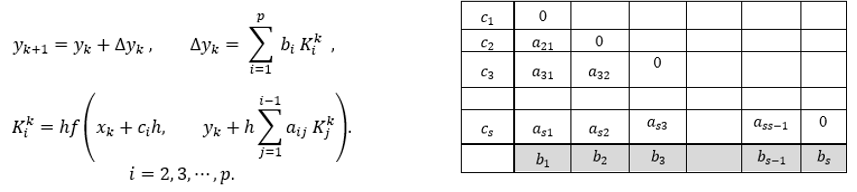
\includegraphics[width=15cm]{2-03-runge}
%     \caption{Общий вид явных схем}
%     \label{fig:Runge}
% \end{figure}

\begin{figure}
    \begin{minipage}[t]{8.5cm}
        {\small
        \begin{equation*}
            \begin{cases}
                y_{k + 1} = y_k + \Delta y_k\\
                \Delta y_k = \sum\limits_{i = 1}^sb_iK_i^k\\
                K_i^k = hf(x_k + c_ih, y_k + h\sum\limits_{j = 1}^{i - 1}a_{ij}K_j^k)
            \end{cases}
            %\label{eq-koshi-system}
        \end{equation*}
        }
    \end{minipage}
    \begin{minipage}[t]{7.5cm}
        \begin{table}    
            %\caption{Таблица Бутчера для метода явного метода Рунге-Кутты 4-го порядка}
            \begin{tabular}{|c|c|c|c|c|c|c|}
            \hline
            $c_1$ & $0$ & $0$ & $0$ & & $0$ & $0$\\
            \hline
            $c_2$ & $a_{21}$ & $0$ & $0$ & & $0$ & $0$\\
            \hline
            $c_3$ & $a_{31}$ & $a_{32}$ & $0$ & & $0$ & $0$\\
            \hline
            & & & & & &\\
            \hline
            $c_s$ & $a_{s1}$ & $a_{s2}$ & $a_{s3}$ & & $a_{ss-1}$ & $0$\\
            \hline
            & \cellcolor{lightgray} $b_1$ & \cellcolor{lightgray} $b_2$ & \cellcolor{lightgray} $b_3$ & \cellcolor{lightgray} & \cellcolor{lightgray} $b_{s-1}$ &  \cellcolor{lightgray} $b_s$\\
            \hline
            \end{tabular}
            %\label{tab:RungeKutta4}
        \end{table}
    \end{minipage}
    \caption{Общий вид явных схем}
    \label{fig:Runge}
\end{figure}

В литературе можно подобрать целую коллекцию одношаговых маршевых многоэтапных методов, которые обеспечивают адекватную точность и
подходят для решения нежёстких ОДУ. Среди этих методов можно выделить классический метод Рунге-Кутты 4-го порядка, представленный на
схеме \ref{fig:RungeKutta4}.

\begin{figure}
\begin{minipage}[t]{8.5cm}
    {\small
    \begin{equation*}
        \begin{cases}
            y_{k + 1} = y_k + \Delta y_k\\
            \Delta y_k = \frac{1}{6} (K_1^k + 2K_2^k + 2K_3^k + K_4^k)\\
            K_1^k = hf(x_k, y_k)\\
            K_2^k = hf(x_k + \frac{1}{2}h, y_k + \frac{1}{2}K_1^k)\\
            K_3^k = hf(x_k + \frac{1}{2}h, y_k + \frac{1}{2}K_2^k)\\
            K_4^k = hf(x_k + h, y_k + K_3^k)
        \end{cases}
        %\label{eq-koshi-system}
    \end{equation*}
    }
\end{minipage}
\begin{minipage}[t]{7.5cm}
    \begin{table}    
        %\caption{Таблица Бутчера для метода явного метода Рунге-Кутты 4-го порядка}
        \begin{tabular}{|c|c|c|c|c|}
        \hline
        $0$ & $0$ & $0$ & $0$ & $0$\\
        \hline
        $\frac{1}{2}$ & $\frac{1}{2}$ & $0$ & $0$ & $0$\\
        \hline
        $\frac{1}{2}$ & $0$ & $\frac{1}{2}$ & $0$ & $0$\\
        \hline
        $1$ & $0$ & $0$ & $1$ & $0$\\
        \hline
        $0$ & \cellcolor{lightgray} $\frac{1}{6}$ & \cellcolor{lightgray} $\frac{1}{3}$ & \cellcolor{lightgray} $\frac{1}{3}$ & \cellcolor{lightgray} $\frac{1}{6}$\\
        \hline
        \end{tabular}
        %\label{tab:RungeKutta4}
    \end{table}
\end{minipage}
\caption{Схема Рунге-Кутты 4-го порядка}
\label{fig:RungeKutta4}
\end{figure}

Для более жёстких задач метод Рунге-Кутты 4-го порядка может быть недостаточно точным. Иногда приходится сильно уменьшать шаг
интегрирования для того, чтобы решение было устойчивым. Другой путь ~--- использование методов более высоких порядков, например метода
Рунге-Кутты 6-го порядка, представленного на схеме \ref{fig:RungeKutta6}

\begin{figure}
    \begin{minipage}[t]{8.5cm}
        {\small
        \begin{equation*}
            \begin{cases}
                y_{k + 1} = y_k + \Delta y_k\\
                \Delta y_k = \frac{7}{90} (K_1^k + K_6^k) + \frac{16}{45} (K_2^k + K_5^k) -\\
                - \frac{1}{3}K_3^k + \frac{7}{15}K_4^k\\
                K_1^k = hf(x_k, y_k)\\
                K_2^k = hf(x_k + \frac{1}{4}h, y_k + \frac{1}{4}K_1^k)\\
                K_3^k = hf(x_k + \frac{1}{2}h, y_k + \frac{1}{2}K_1^k)\\
                K_4^k = hf(x_k + \frac{1}{2}h, y_k + \frac{1}{7}K_1^k + \frac{2}{7}K_2^k +\\
                + \frac{1}{14}K_3^k)\\
                K_5^k = hf(x_k + \frac{3}{4}h, y_k + \frac{3}{8}K_1^k - \frac{1}{2}K_3^k +\\
                + \frac{7}{8}K_4^k)\\
                K_6^k = hf(x_k + h, y_k - \frac{4}{7}K_1^k + \frac{12}{7}K_2^k -\\
                - \frac{2}{7}K_3^k - K_4^k + \dfrac{8}{7}K_5^k)
            \end{cases}
            %\label{eq-koshi-system}
        \end{equation*}
        }
    \end{minipage}
    \begin{minipage}[t]{7.5cm}
        \begin{table}    
            %\caption{Таблица Бутчера для метода явного метода Рунге-Кутты 6-го порядка}
            \begin{tabular}{|c|c|c|c|c|c|c|}
            \hline
            $0$ & $0$ & $0$ & $0$ & $0$ & $0$ & $0$\\
            \hline
            $\frac{1}{4}$ & $\frac{1}{4}$ & $0$ & $0$ & $0$ & $0$ & $0$\\
            \hline
            $\frac{1}{2}$ & $\frac{1}{2}$ & $0$ & $0$ & $0$ & $0$ & $0$\\
            \hline
            $\frac{1}{2}$ & $\frac{1}{7}$ & $\frac{2}{7}$ & $\frac{1}{14}$ & $0$ & $0$ & $0$\\
            \hline
            $\frac{3}{4}$ & $\frac{3}{8}$ & $0$ & $-\frac{1}{2}$ & $\frac{7}{8}$ & $0$ & $0$\\
            \hline
            $1$ & $-\frac{4}{7}$ & $\frac{12}{7}$ & $-\frac{2}{7}$ & $-1$ & $7$ & $0$\\
            \hline
            $0$ & \cellcolor{lightgray} $\frac{7}{90}$ & \cellcolor{lightgray} $\frac{16}{45}$ & \cellcolor{lightgray} $-\frac{1}{3}$ & \cellcolor{lightgray} $\frac{7}{15}$ & \cellcolor{lightgray} $\frac{16}{45}$ & \cellcolor{lightgray} $\frac{7}{90}$\\
            \hline
            \end{tabular}
            %\label{tab:RungeKutta6}
        \end{table}
    \end{minipage}
    \caption{Схема Рунге-Кутты 6-го порядка}
    \label{fig:RungeKutta6}
\end{figure}

\subsection{Явные вложенные схемы для решения ОДУ}

В связи с перечисленными недостатками обычных явных схем, есть смысл применить явные вложенные схемы, которые базируются так же на
нижней треугольной матрице Бутчера, обладают маршевым
методом решения и позволяют на базе одних и тех же поправочных коэффициентов моделировать решение с разным порядком точности и тем
самым либо увеличивать шаг интегрирования, либо уменьшать. Общий вид этих схем отличается от явных лишь наличием дополнительной строки
в таблице Бутчера, по которая и позволяет моделировать решение с другим порядком точности для сравнения погрешности. На рисунке
\ref{fig:Falberg} представлен общий вид явных вложенных схем.

% \begin{figure}
%     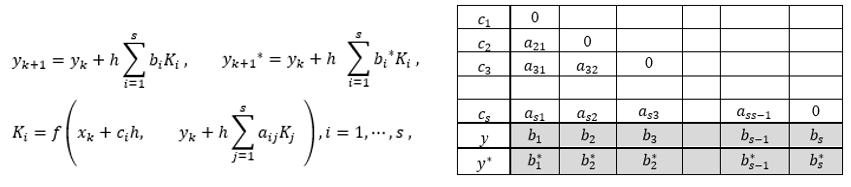
\includegraphics[width=15cm]{2-03-falberg}
%     \caption{Общий вид явных вложенных схем}
%     \label{fig:Falberg}
% \end{figure}

\begin{figure}
    \begin{minipage}[t]{8.5cm}
        {\small
        \begin{equation*}
            \begin{cases}
                y_{k + 1} = y_k + \sum\limits_{i = 1}^sb_iK_i^k\\
                y_{k + 1}^* = y_k + \sum\limits_{i = 1}^sb_i^*K_i^k\\
                K_i^k = hf(x_k + c_ih, y_k + h\sum\limits_{j = 1}^{i - 1}a_{ij}K_j^k)
            \end{cases}
            %\label{eq-koshi-system}
        \end{equation*}
        }
    \end{minipage}
    \begin{minipage}[t]{7.5cm}
        \begin{table}    
            %\caption{Таблица Бутчера для метода явного метода Рунге-Кутты 4-го порядка}
            \begin{tabular}{|c|c|c|c|c|c|c|}
            \hline
            $c_1$ & $0$ & $0$ & $0$ & & $0$ & $0$\\
            \hline
            $c_2$ & $a_{21}$ & $0$ & $0$ & & $0$ & $0$\\
            \hline
            $c_3$ & $a_{31}$ & $a_{32}$ & $0$ & & $0$ & $0$\\
            \hline
            & & & & & &\\
            \hline
            $c_s$ & $a_{s1}$ & $a_{s2}$ & $a_{s3}$ & & $a_{ss-1}$ & $0$\\
            \hline
            & \cellcolor{lightgray} $b_1$ & \cellcolor{lightgray} $b_2$ & \cellcolor{lightgray} $b_3$ & \cellcolor{lightgray} & \cellcolor{lightgray} $b_{s-1}$ &  \cellcolor{lightgray} $b_s$\\
            \hline
            & \cellcolor{lightgray} $b_1^*$ & \cellcolor{lightgray} $b_2^*$ & \cellcolor{lightgray} $b_3^*$ & \cellcolor{lightgray} & \cellcolor{lightgray} $b_{s-1}^*$ &  \cellcolor{lightgray} $b_s^*$\\
            \hline
            \end{tabular}
            %\label{tab:RungeKutta4}
        \end{table}
    \end{minipage}
    \caption{Общий вид явных вложенных схем}
    \label{fig:Falberg}
\end{figure}

Порядок точности таких схем записывется в виде $n(m)$, где $n$ ~--- порядок схемы при использовании верхней строки коэффициентов
$b$, $m$ ~--- нижней. Если разница в решениях при использовании этих порядков высока, то шаг следует уменьшить, если же наоборот ~---
разница очень низкая, то шаг можно увеличить для ускорения работы алгоритма.
Пример схемы для метода Фалберга 2(3)-го порядка \ref{fig:Falberg2}:

\begin{figure}
    \begin{minipage}[t]{8.5cm}
        {\small
        \begin{equation*}
            \begin{cases}
                y_{k + 1} = y_k + \frac{1}{2}K_1^k + \frac{1}{2}K_2^k\\
                y^{*}_{k + 1} = y_k + \frac{1}{2}K_1^k + \frac{1}{2}K_2^k\\
                K_1^k = hf(x_k, y_k)\\
                K_2^k = hf(x_k + h, y_k + K_1^k)\\
                K_3^k = hf(x_k + \frac{1}{2}h, y_k + \frac{1}{4}K_1^k + \frac{1}{4}K_2^k)\\
                R = |y_{k + 1} - y^{*}_{k + 1}|
            \end{cases}
            %\label{eq-koshi-system}
        \end{equation*}
        }
    \end{minipage}
    \begin{minipage}[t]{7.5cm}
        \begin{table}
            %\caption{Схема метода Фалберга 2(3)-го порядка}
            \begin{tabular}{|c|c|c|c|}
            \hline
            $0$ & $0$ & $0$ & $0$\\
            \hline
            $1$ & $1$ & $0$ & $0$\\
            \hline
            $\frac{1}{2}$ & $\frac{1}{4}$ & $\frac{1}{4}$ & $0$\\
            \hline
            $0$ & \cellcolor{lightgray} $\frac{1}{2}$ & \cellcolor{lightgray} $\frac{1}{2}$ & \cellcolor{lightgray} $0$\\
            \hline
            $0$ & \cellcolor{lightgray} $\frac{1}{6}$ & \cellcolor{lightgray} $\frac{1}{6}$ & \cellcolor{lightgray} $\frac{4}{6}$\\
            \hline
            \end{tabular}
            %\label{tab:Falberg2}
        \end{table}
    \end{minipage}
    \caption{Схема Фалберга 2(3)-го порядка}
    \label{fig:Falberg2}
\end{figure}

Среди вложенных методов выделяется Дорман-Принц 4(5)-го порядка, который является наиболее популярным в этой гркппе методов.
Таблица Бутчера
для метода Дормана-Принца \ref{tab:DormanPrince45} обладает большим размером и состоит в основном из громоздких дробей. Стоит отметить,
что последний этап этого метода
рассчитывается в той же точке, что и первый этап следующего шага, что позволяет сэкономить немного времи на вычислениях.

\begin{table}    
    \caption{Таблица Бутчера для метода Дормана-Принца 4(5)-го порядка}
    \begin{tabular}{|c|c|c|c|c|c|c|c|}
    \hline
    $0$ & $0$ & $0$ & $0$ & $0$ & $0$ & $0$ & $0$\\
    \hline
    $\frac{1}{5}$ & $\frac{1}{5}$ & $0$ & $0$ & $0$ & $0$ & $0$ & $0$\\
    \hline
    $\frac{3}{10}$ & $\frac{3}{40}$ & $\frac{9}{40}$ & $0$ & $0$ & $0$ & $0$ & $0$\\
    \hline
    $\frac{4}{5}$ & $\frac{44}{45}$ & $-\frac{56}{15}$ & $\frac{32}{9}$ & $0$ & $0$ & $0$ & $0$\\
    \hline
    $\frac{8}{9}$ & $\frac{19372}{6561}$ & $-\frac{25360}{2187}$ & $\frac{64448}{6561}$ & $-\frac{212}{729}$ & $0$ & $0$ & $0$\\
    \hline
    $1$ & $\frac{9017}{3168}$ & $-\frac{355}{33}$ & $\frac{46732}{5247}$ & $\frac{49}{176}$ & $-\frac{5103}{18656}$ & $0$ & $0$\\
    \hline
    $1$ & $\frac{35}{384}$ & $0$ & $\frac{500}{1113}$ & $\frac{125}{192}$ & $-\frac{2187}{6784}$ & $\frac{11}{84}$ & $0$\\
    \hline
    $0$ & \cellcolor{lightgray} $\frac{35}{384}$ & \cellcolor{lightgray} $0$ & \cellcolor{lightgray} $\frac{500}{1113}$ & \cellcolor{lightgray} $\frac{125}{192}$ & \cellcolor{lightgray} $-\frac{2187}{6784}$ & \cellcolor{lightgray} $\frac{11}{84}$ & \cellcolor{lightgray} $0$\\
    \hline
    $0$ & \cellcolor{lightgray} $\frac{5179}{57600}$ & \cellcolor{lightgray} $0$ & \cellcolor{lightgray} $\frac{7571}{16695}$ & \cellcolor{lightgray} $\frac{393}{640}$ & \cellcolor{lightgray} $-\frac{92097}{339200}$ & \cellcolor{lightgray} $\frac{187}{2100}$ & \cellcolor{lightgray} $\frac{1}{40}$\\
    \hline
    \end{tabular}
    \label{tab:DormanPrince45}
\end{table}

Разработано множество вложенных многоэтапных методов, но для решения сложных задач представляют интерес методы, обладающие минимальным
числом этапов и максимальным порядком точности.

\subsection{Неявные схемы для решения ОДУ}

К наиболее сложным методам можно отнести группу неявных схем. Плотно заполненная таблица Бутчера не позволяет использовать маршевые
методы и принуждает решать систему алгебраических уравнений на каждом шаге интегрирования, что вызывет определённые сложности у
разработчиков.

% \begin{figure}
%     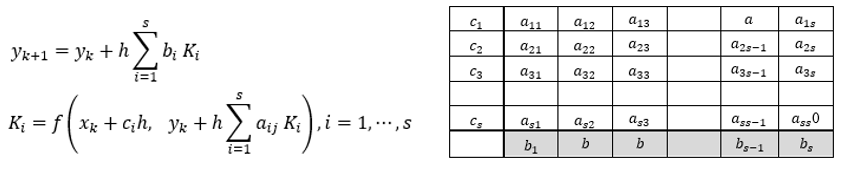
\includegraphics[width=15cm]{2-03-gauss}
%     \caption{Общий вид неявных схем}
%     \label{fig:Gauss}
% \end{figure}

\begin{figure}
    \begin{minipage}[t]{8.5cm}
        {\small
        \begin{equation*}
            \begin{cases}
                y_{k + 1} = y_k + \sum\limits_{i = 1}^sb_iK_i^k\\
                K_i^k = hf(x_k + c_ih, y_k + h\sum\limits_{j = 1}^{s}a_{ij}K_j^k)
            \end{cases}
            %\label{eq-koshi-system}
        \end{equation*}
        }
    \end{minipage}
    \begin{minipage}[t]{7.5cm}
        \begin{table}    
            %\caption{Таблица Бутчера для метода явного метода Рунге-Кутты 4-го порядка}
            \begin{tabular}{|c|c|c|c|c|c|c|}
            \hline
            $c_1$ & $a_{11}$ & $a_{12}$ & $a_{13}$ & & $a_{1s-1}$ & $a_{1s}$\\
            \hline
            $c_2$ & $a_{21}$ & $a_{22}$ & $a_{23}$ & & $a_{2s-1}$ & $a_{2s}$\\
            \hline
            $c_3$ & $a_{31}$ & $a_{32}$ & $a_{33}$ & & $a_{3s-1}$ & $a_{3s}$\\
            \hline
            & & & & & &\\
            \hline
            $c_s$ & $a_{s1}$ & $a_{s2}$ & $a_{s3}$ & & $a_{ss-1}$ & $a_{ss}$\\
            \hline
            & \cellcolor{lightgray} $b_1$ & \cellcolor{lightgray} $b_2$ & \cellcolor{lightgray} $b_3$ & \cellcolor{lightgray} & \cellcolor{lightgray} $b_{s-1}$ &  \cellcolor{lightgray} $b_s$\\
            \hline
            \end{tabular}
            %\label{tab:RungeKutta4}
        \end{table}
    \end{minipage}
    \caption{Общий вид неявных схем}
    \label{fig:Gauss}
\end{figure}

Особенностью этих методов является то, что в качестве базовых опорных точек являются иррациональные корни многочлена Лежанра.
На схеме \ref{fig:Gauss4} показан неявный метод Гаусса 4-го порядка.

\begin{figure}
    \begin{minipage}[t]{8.5cm}
        {\small
        \begin{equation*}
            \begin{cases}
                y_{k + 1} = y_k + \frac{1}{2}hK_1 + \frac{1}{2}hK_2\\
                K_1 = f(x_k + h(\frac{1}{2} - \frac{\sqrt{3}}{6}), y_k + \frac{1}{4}hK_1 +\\
                + (\frac{1}{4} - \frac{\sqrt{3}}{6})hK_2)\\
                K_2 = f(x_k + h(\frac{1}{2} + \frac{\sqrt{3}}{6}), y_k + (\frac{1}{4} + \frac{\sqrt{3}}{6})hK_1 +\\
                + \frac{1}{4}hK_2)
            \end{cases}
            %\label{eq-koshi-system}
        \end{equation*}
        }
    \end{minipage}
    \begin{minipage}[t]{7.5cm}
        \begin{table}    
            %\caption{Таблица Бутчера для метода неявного метода Гаусса 4-го порядка}
            \begin{tabular}{|c|c|c|}
            \hline
            $\frac{1}{2} - \frac{\sqrt{3}}{6}$ & $\frac{1}{4}$ & $\frac{1}{4} - \frac{\sqrt{3}}{6}$\\
            \hline
            $\frac{1}{2} + \frac{\sqrt{3}}{6}$ & $\frac{1}{4} + \frac{\sqrt{3}}{6}$ & $\frac{1}{4}$\\
            \hline
            $0$ & \cellcolor{lightgray} $\frac{1}{2}$ & \cellcolor{lightgray} $\frac{1}{2}$\\
            \hline
            \end{tabular}
            %\label{tab:Gauss4}
        \end{table}
    \end{minipage}
    \caption{Схема неявного Гаусса 4-го порядка}
    \label{fig:Gauss4}
\end{figure}

По схеме видно, что для нахождения коэффициентов $K_i$ обычные маршевые методы не подходят. Для их получения нужно использовать
итерационные методы, такие как метод простой итерации, метод Зейделя и метод Ньютона. Таблицы Бутчера неявных методов обладают
меньшим размером по сравнению с явными, сохраняя тот же порядок точности. Хорошим примером копактности послужит
таблица \ref{tab:Gauss6}, неявного метода Гаусса 6-го порядка.

\begin{table}    
    \caption{Таблица Бутчера для метода неявного метода Гаусса 6-го порядка}
    \begin{tabular}{|c|c|c|c|}
    \hline
    $\frac{1}{2} - \frac{\sqrt{15}}{10}$ & $\frac{5}{36}$ & $\frac{2}{9} - \frac{\sqrt{15}}{15}$ & $\frac{5}{36} - \frac{\sqrt{15}}{30}$\\
    \hline
    $\frac{1}{2}$ & $\frac{5}{36} + \frac{\sqrt{15}}{24}$ & $\frac{2}{9}$ & $\frac{5}{36} - \frac{\sqrt{15}}{24}$\\
    \hline
    $\frac{1}{2} + \frac{\sqrt{15}}{10}$ & $\frac{5}{36} + \frac{\sqrt{15}}{30}$ & $\frac{2}{9} + \frac{\sqrt{15}}{15}$ & $\frac{5}{36}$\\
    \hline
    $0$ & \cellcolor{lightgray} $\frac{5}{18}$ & \cellcolor{lightgray} $\frac{4}{9}$ & \cellcolor{lightgray} $\frac{5}{18}$\\
    \hline
    \end{tabular}
    \label{tab:Gauss6}
\end{table}

Помимо перечисленных групп методов, существуют так же диагональные неявные методы, неявные вложенные, неявные методы без одной строки
или столбца, но все они являются подгруппами неявных методов и используют тот же вид общей схемы. Отдельно можно уделить внимание
диагональным методам.

\subsection{Полунеявные схемы для решения ОДУ}

Полунеявные или диагональные схемы входят в группу неявных методо, имеют нижнюю треугольную форму таблицы Бутчера и ненулевыми
элементами диагонали. Данная особенность позволяет решать системы уравнений для поиска $K_i$ при помощи распараллеливания, что гораздо
быстрее на многоядерных процессорах, а так же с использованием не более одной итерации. К недостаткам таких схем относится плохая
устойчивость по сравнению с обычными неявными.

В качестве примера таких схем можно привести Диагональный метод 4-го порядка, представленный на схеме \ref{fig:Diagonal4}

\begin{figure}
    \begin{minipage}[t]{8.5cm}
        {\small
        \begin{equation*}
            \begin{cases}
                y_{k + 1} = y_k - hK_1 + \frac{3}{2}hK_2 - hK_3 + \frac{3}{2}hK_4\\
                K_1 = f(x_k + \frac{1}{2}h, y_k + \frac{1}{2}hK_1)\\
                K_2 = f(x_k + \frac{2}{3}h, y_k + \frac{2}{3}hK_2)\\
                K_3 = f(x_k + \frac{1}{2}h, y_k - \frac{5}{2}hK_1 + \frac{5}{2}hK_2 - \frac{1}{2}hK_3)\\
                K_4 = f(x_k + \frac{1}{3}h, y_k - \frac{5}{3}hK_1 + \frac{4}{3}hK_2 - \frac{2}{3}hK_4)\\
            \end{cases}
            %\label{eq-koshi-system}
        \end{equation*}
        }
    \end{minipage}
    \begin{minipage}[t]{7.5cm}
        \begin{table}    
            %\caption{Таблица Бутчера для метода неявного метода Гаусса 4-го порядка}
            \begin{tabular}{|c|c|c|c|c|}
            \hline
            $\frac{1}{2}$ & $\frac{1}{2}$ & $0$ & $0$ & $0$\\
            \hline
            $\frac{2}{3}$ & $0$ & $\frac{2}{3}$ & $0$ & $0$\\
            \hline
            $\frac{1}{2}$ & $-\frac{5}{2}$ & $\frac{5}{2}$ & $\frac{1}{2}$ & $0$\\
            \hline
            $\frac{1}{3}$ & $-\frac{5}{3}$ & $\frac{4}{3}$ & $0$ & $\frac{2}{3}$\\
            \hline
            $0$ & \cellcolor{lightgray} $-1$ & \cellcolor{lightgray} $\frac{3}{2}$ & \cellcolor{lightgray} $-1$ & \cellcolor{lightgray} $\frac{3}{2}$\\
            \hline
            \end{tabular}
            %\label{tab:Gauss4}
        \end{table}
    \end{minipage}
    \caption{Схема Диагонального метода 4-го порядка}
    \label{fig:Diagonal4}
\end{figure}

Преимущество явных методов заключается в производительности, так как им не нужно решать на каждом шаге системы алгебраических
уравнений. Отсюда следует, что использование явных методов даёт больший выигрыш по времени, чем использование более производительного
оборудования и распараллеливания. Главным же преимуществом неявных методов является наличие устойчивости (А-устойчивости, L-устойчивости и
так далее), в результате чего полученное ими решение является гарантированно устойчивым, в отличие от явных.

\subsection{Устойчивость}

Текст

%критерии устойчивости

Однако некоторые СДУ, описывающие химические процессы можно решить и явными методами с требуемой точностью, потому что свойства А и
L-устойчивости являются
лишь достаточным, но не необходимым условием эффективности решения, поэтому нельзя использовать только те или иные методы. Выбрать
оптимальный метод можно путём целевого тестирования.

\subsection{Решение систем алгебраических уравнений}

Теперь рассмотрим алгоритмы решения систем алгебраических уравнений для итерационных процессов в неявных методах. В данной работе
реализовано 3 таких алгоритма:
\begin{itemize}
    \item метод простой итерации,
    \item метод Зейделя,
    \item метод Ньютона.
\end{itemize}

Метод Зейделя и простой итерации являются достаточно быстрыми алгоритмами, так как им не нужно дифференцировать функции или
вычислять Якобиан. Отличие метода Зейделя от метода простой итерации заключается в том, что при вычислении очередного приближения
вектора неизвестных используются уже уточненные значения на этом же шаге итерации. Это обеспечивает более быструю сходимость метода
Зейделя. Общий вид метода простой итерации и Зейделя представлен в формулах \ref{eq:SI} и \ref{eq:Zeidel} соответственно.

% \begin{figure}
%     \begin{minipage}[t]{8.5cm}
%         {\small
%         \begin{equation*}
%             \begin{cases}
%                 y_{k + 1} = y_k - hK_1 + \frac{3}{2}hK_2 - hK_3 + \frac{3}{2}hK_4\\
%                 K_1 = f(x_k + \frac{1}{2}h, y_k + \frac{1}{2}hK_1)\\
%                 K_2 = f(x_k + \frac{2}{3}h, y_k + \frac{2}{3}hK_2)\\
%                 K_3 = f(x_k + \frac{1}{2}h, y_k - \frac{5}{2}hK_1 + \frac{5}{2}hK_2 - \frac{1}{2}hK_3)\\
%                 K_4 = f(x_k + \frac{1}{3}h, y_k - \frac{5}{3}hK_1 + \frac{4}{3}hK_2 - \frac{2}{3}hK_4)\\
%             \end{cases}
%             %\label{eq-koshi-system}
%         \end{equation*}
%         }
%     \end{minipage}
%     \begin{minipage}[t]{7.5cm}
%         {\small
%         \begin{equation*}
%             \begin{cases}
%                 y_{k + 1} = y_k - hK_1 + \frac{3}{2}hK_2 - hK_3 + \frac{3}{2}hK_4\\
%                 K_1 = f(x_k + \frac{1}{2}h, y_k + \frac{1}{2}hK_1)\\
%                 K_2 = f(x_k + \frac{2}{3}h, y_k + \frac{2}{3}hK_2)\\
%                 K_3 = f(x_k + \frac{1}{2}h, y_k - \frac{5}{2}hK_1 + \frac{5}{2}hK_2 - \frac{1}{2}hK_3)\\
%                 K_4 = f(x_k + \frac{1}{3}h, y_k - \frac{5}{3}hK_1 + \frac{4}{3}hK_2 - \frac{2}{3}hK_4)\\
%             \end{cases}
%             %\label{eq-koshi-system}
%         \end{equation*}
%         }
%     \end{minipage}
%     \caption{Схема Диагонального метода 4-го порядка}
%     \label{fig:Diagonal4}
% \end{figure}

% \begin{figure}
%     \begin{subfigure}[t]{0.45\linewidth}
%         \centering
%         {\small
%             $K_i^{j + 1} = f(x_k + c_ih, y_k + a_{i1}hK_1^{j} + a_{i2}hK_2^{j} + ... a_{ii}hK_i^{j} + ... + a_{is}hK_s^{j})$
%         }
%         \caption{}
%     \end{subfigure}
%     \hfill
%     \begin{subfigure}[t]{0.45\linewidth}
%         \centering
%         {\small
%             $K_i^{j + 1} = f(x_k + c_ih, y_k + a_{i1}hK_1^{j + 1} + a_{i2}hK_2^{j + 1} + ... a_{ii}hK_i^{j} + ... + a_{is}hK_s^{j})$
%         }
%         \caption{}
%     \end{subfigure}
%     \hfill
%     \caption{Схемы методов решения САУ: а) простой итерации; б) Зейделя}
%     \label{fig:bomb}
% \end{figure}

\begin{equation}
    K_i^{j + 1} = f(x_k + c_ih, y_k + a_{i1}hK_1^{j} + a_{i2}hK_2^{j} + ... a_{ii}hK_i^{j} + ... + a_{is}hK_s^{j})
    \label{eq:SI}
\end{equation}

\begin{equation}
    K_i^{j + 1} = f(x_k + c_ih, y_k + a_{i1}hK_1^{j + 1} + a_{i2}hK_2^{j + 1} + ... a_{ii}hK_i^{j} + ... + a_{is}hK_s^{j})
    \label{eq:Zeidel}
\end{equation}

В качестве начальных приближений можно взять значения $K$ с предыдущего шага. Для первого же шага можно посчитать значения $K$ явными
методами.

Более интересным для рассмотрения является метод Ньютона (\ref{eq:Newton}). Медленная скорость работы, обусловленная необходимостью строить матрицу Якоби
на каждом шаге итерирования, позволяет получать решение устойчиво независимо от начального приближения $K$.

\begin{equation}
    \begin{gathered}
        \begin{pmatrix}
            K_1^{j + 1}\\
            K_2^{j + 1}\\
            ...\\
            K_s^{j + 1}
        \end{pmatrix}
        =
        \begin{pmatrix}
            K_1^{j}\\
            K_2^{j}\\
            ...\\
            K_s^{j}
        \end{pmatrix}
        -
        \begin{pmatrix}
            \frac{\partial F_1}{\partial K_1} & \frac{\partial F_1}{\partial K_2} & ... & \frac{\partial F_1}{\partial K_s}\\
            \frac{\partial F_2}{\partial K_1} & \frac{\partial F_2}{\partial K_2} & ... & \frac{\partial F_2}{\partial K_s}\\
            ...\\
            \frac{\partial F_s}{\partial K_1} & \frac{\partial F_s}{\partial K_2} & ... & \frac{\partial F_s}{\partial K_s}\\
        \end{pmatrix}
        \times
        \begin{pmatrix}
            F_1\\
            F_2\\
            ...\\
            F_s
        \end{pmatrix}\\
        F_i = K_i^j - f(x_k + c_ih, y_k + a_{i1}hK_1^{j} + a_{i2}hK_2^{j} + ... a_{ii}hK_i^{j} + ... + a_{is}hK_s^{j})
    \end{gathered}
    \label{eq:Newton}
\end{equation}

Несмотря на лучшую сходимость решения, в большинстве случаев для решения уравнений химической кинетики было достаточно использовать
методы простой итерации и Зейделя, так как они быстрее. В случаях, когда их было недостаточно, применялся метод Ньютона. 
Для построения матрицы Якоби сначала строятся функции $F_i$, после чего используются алгоритмы численного дифференцирования с
различным порядком точности.

\subsection{Дифференцирование}

Дифференцирование ~--- операция взятия полной или частной производной функции. В работе было реализовано 4 метода
дифференцирования первого порядка: 2-х точечный, 3-х точечный и два 4-х точечных.

\begin{equation}
    \begin{gathered}
        y_i' = \frac{y_{i+1} - y_{i-1}}{2h}\\
        y_i' = \frac{-3y_{i} + 4y_{i+1} - y_{i+2}}{2h}\\
        y_i' = \frac{-y_{i+2} + 8y_{i+1} - 8y_{i-1} + y_{i-2}}{12h}\\
        y_i' = \frac{-11y_{i} + 18y_{i+1} - 9y_{i+2} + 2y_{i+3}}{6h}
    \end{gathered}
    \label{eq:Diff}
\end{equation}

Для метода Ньютона использовалась симметричная формула дифференцирования по 4-м точкам.